\documentclass[11pt]{article}
\usepackage[textwidth=18.0cm, textheight=23.0cm, top=2.0cm]{geometry}
\usepackage{pst-all}
\usepackage{amssymb}
\usepackage{tikz}
\usepackage{underscore}\begin{document}
\pagestyle{empty}


ClassName: \underline{\textbf{Class_10.2bp-6}}
\par
BinSize: \underline{\textbf{100 × 100}}
\par
ReduceSize: \underline{\textbf{100 × 100}}
\par
TypeNum: \underline{\textbf{20}}
\par
Num: \underline{\textbf{20}}
\par
OutS: \underline{\textbf{50000}}
\par
InS: \underline{\textbf{39300}}
\par
Rate: \underline{\textbf{0.786}}
\par
UB: \underline{\textbf{5}}
\par
LB0: \underline{\textbf{5}}
\par
LB: \underline{\textbf{5}}
\par
LBWithCut: \underline{\textbf{5}}
\par
NodeCut: \underline{\textbf{0}}
\par
ExtendedNodeCnt: \underline{\textbf{1}}
\par
GenNodeCnt: \underline{\textbf{1}}
\par
PrimalNode: \underline{\textbf{0}}
\par
ColumnCount: \underline{\textbf{5}}
\par
TotalCutCount: \underline{\textbf{0}}
\par
RootCutCount: \underline{\textbf{0}}
\par
LPSolverCnt: \underline{\textbf{1}}
\par
PricingSolverCnt: \underline{\textbf{0}}
\par
BranchAndBoundNum: \underline{\textbf{1}}
\par
isOpt: \underline{\textbf{true}}
\par
TimeOnInitSolution: \underline{\textbf{0.000 s}}
\par
TimeOnPrimal: \underline{\textbf{0.000 s}}
\par
TimeOnPricing: \underline{\textbf{0.000 s}}
\par
TimeOnRmp: \underline{\textbf{0.063 s}}
\par
TotalTime: \underline{\textbf{0.126 s}}
\par
\newpage


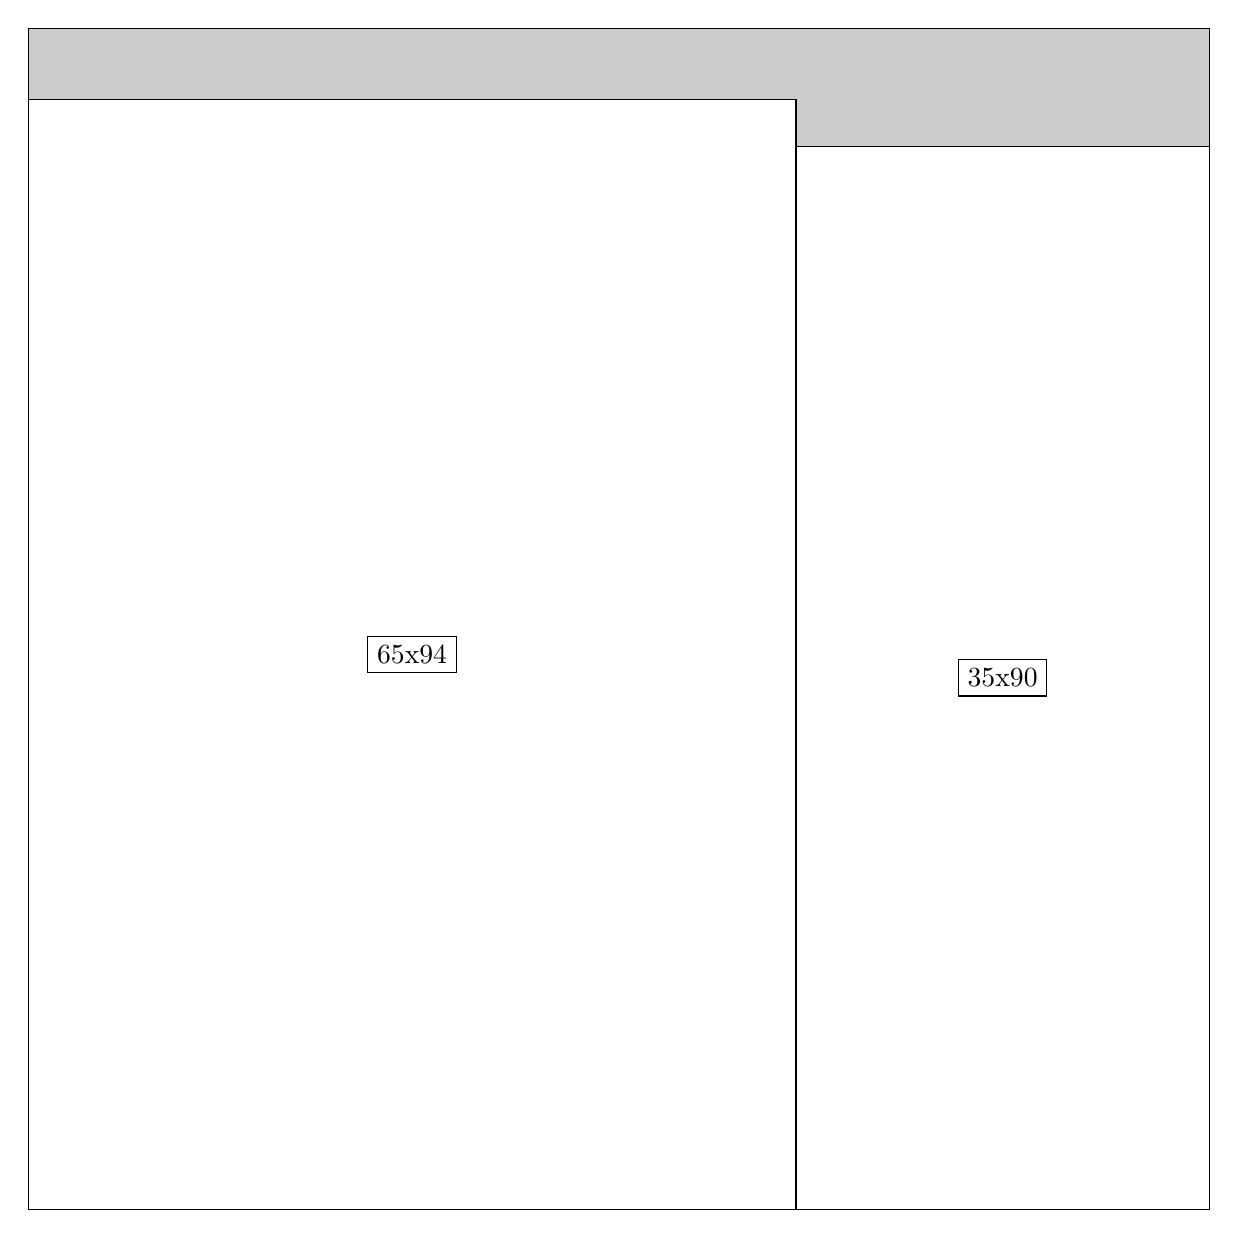
\begin{tikzpicture}[shorten >=1pt,scale=1.0,every node/.style={scale=1.0},->]
\tikzstyle{vertex}=[circle,fill=black!25,minimum size=14pt,inner sep=0pt]
\filldraw[fill=gray!40!white, draw=black] (0,0) rectangle (15.0,15.0);
\foreach \name/\x/\y/\w/\h in {65x94/0.0/0.0/9.75/14.1,35x90/9.75/0.0/5.25/13.5}
\filldraw[fill=white!40!white, draw=black] (\x,\y) rectangle node[draw] (\name) {\name} ++(\w,\h);
\end{tikzpicture}


w =65 , h =94 , x =0 , y =0 , v =6110
\par
w =35 , h =90 , x =65 , y =0 , v =3150
\par
\newpage


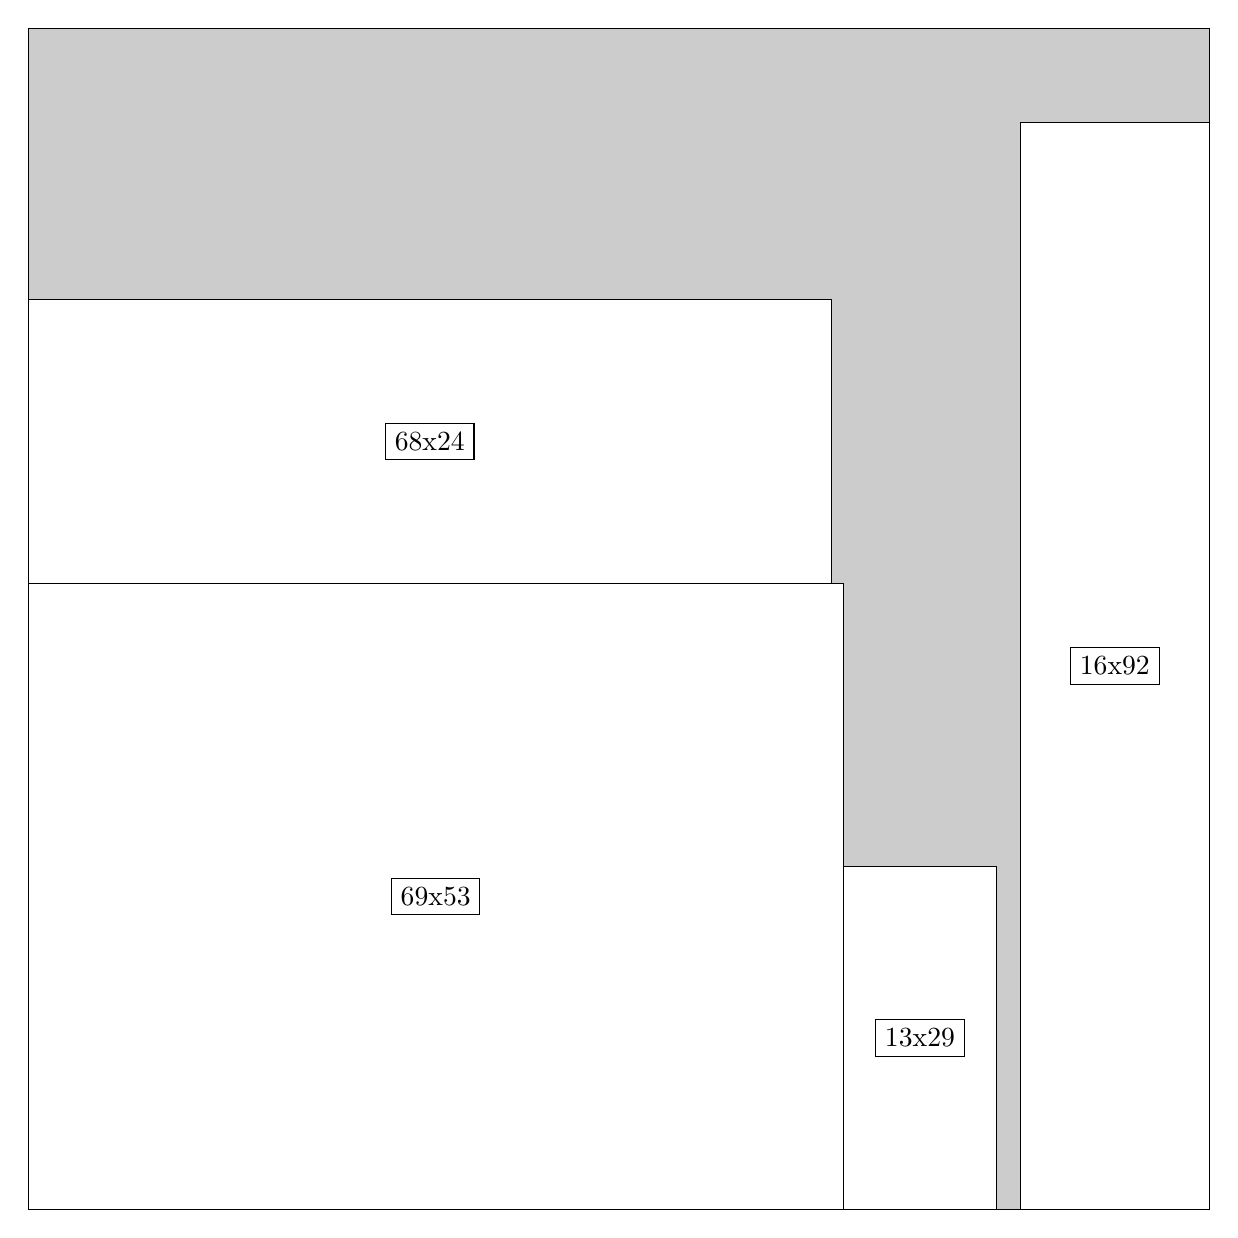
\begin{tikzpicture}[shorten >=1pt,scale=1.0,every node/.style={scale=1.0},->]
\tikzstyle{vertex}=[circle,fill=black!25,minimum size=14pt,inner sep=0pt]
\filldraw[fill=gray!40!white, draw=black] (0,0) rectangle (15.0,15.0);
\foreach \name/\x/\y/\w/\h in {69x53/0.0/0.0/10.35/7.949999999999999,68x24/0.0/7.949999999999999/10.2/3.5999999999999996,16x92/12.6/0.0/2.4/13.799999999999999,13x29/10.35/0.0/1.95/4.35}
\filldraw[fill=white!40!white, draw=black] (\x,\y) rectangle node[draw] (\name) {\name} ++(\w,\h);
\end{tikzpicture}


w =69 , h =53 , x =0 , y =0 , v =3657
\par
w =68 , h =24 , x =0 , y =53 , v =1632
\par
w =16 , h =92 , x =84 , y =0 , v =1472
\par
w =13 , h =29 , x =69 , y =0 , v =377
\par
\newpage


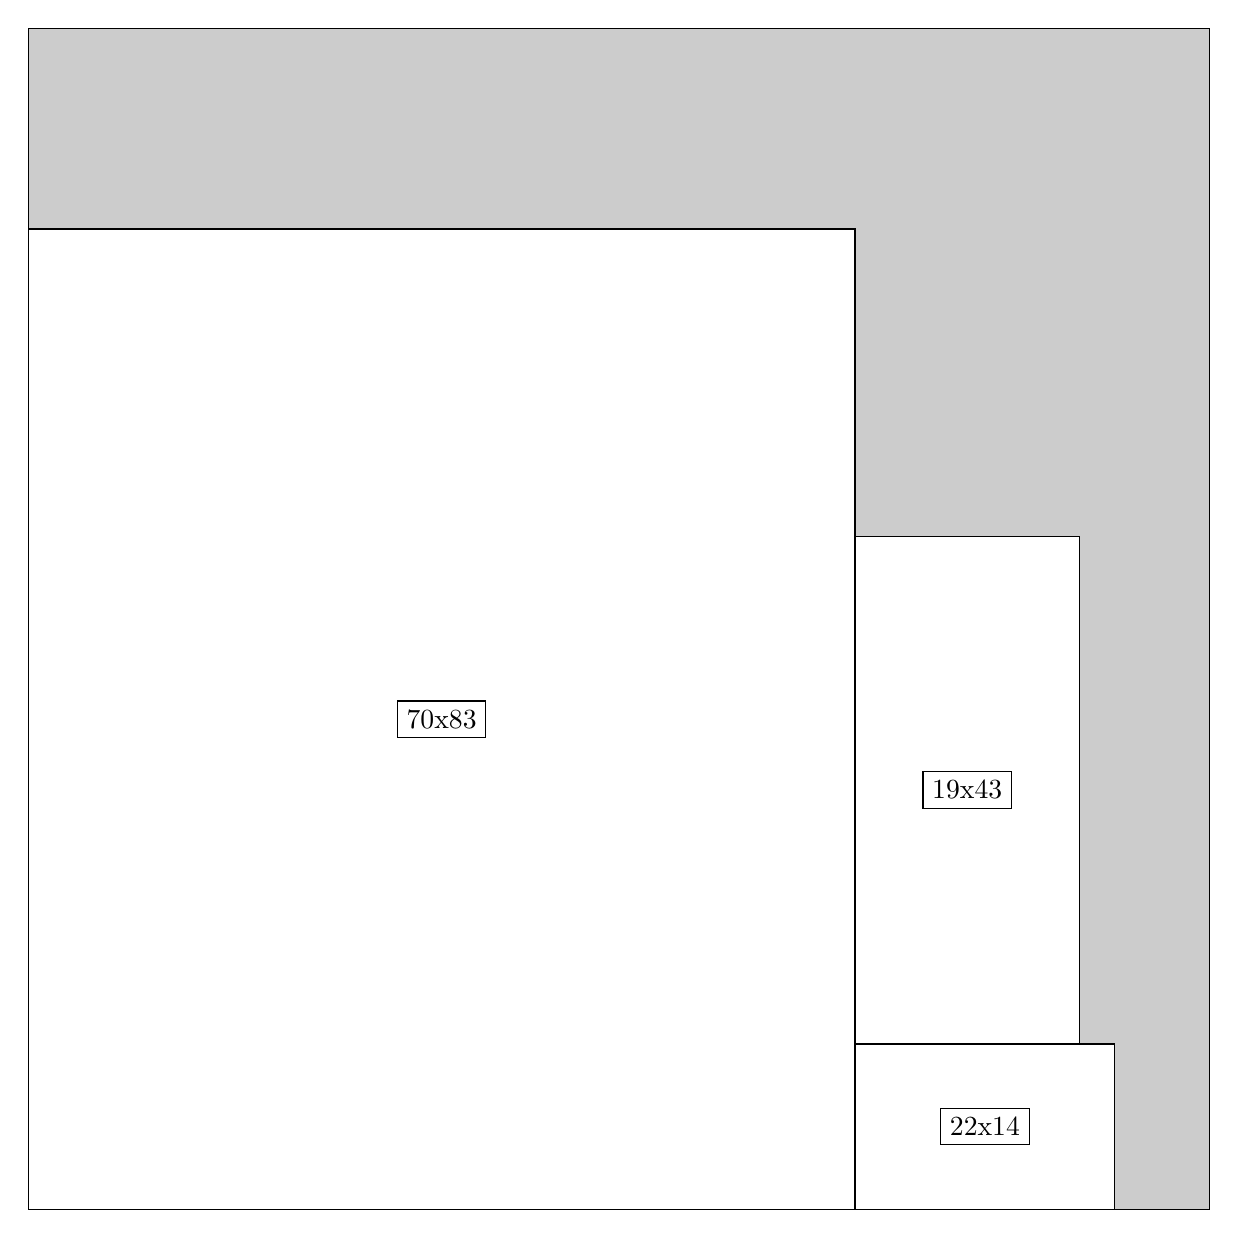
\begin{tikzpicture}[shorten >=1pt,scale=1.0,every node/.style={scale=1.0},->]
\tikzstyle{vertex}=[circle,fill=black!25,minimum size=14pt,inner sep=0pt]
\filldraw[fill=gray!40!white, draw=black] (0,0) rectangle (15.0,15.0);
\foreach \name/\x/\y/\w/\h in {70x83/0.0/0.0/10.5/12.45,19x43/10.5/2.1/2.85/6.45,22x14/10.5/0.0/3.3/2.1}
\filldraw[fill=white!40!white, draw=black] (\x,\y) rectangle node[draw] (\name) {\name} ++(\w,\h);
\end{tikzpicture}


w =70 , h =83 , x =0 , y =0 , v =5810
\par
w =19 , h =43 , x =70 , y =14 , v =817
\par
w =22 , h =14 , x =70 , y =0 , v =308
\par
\newpage


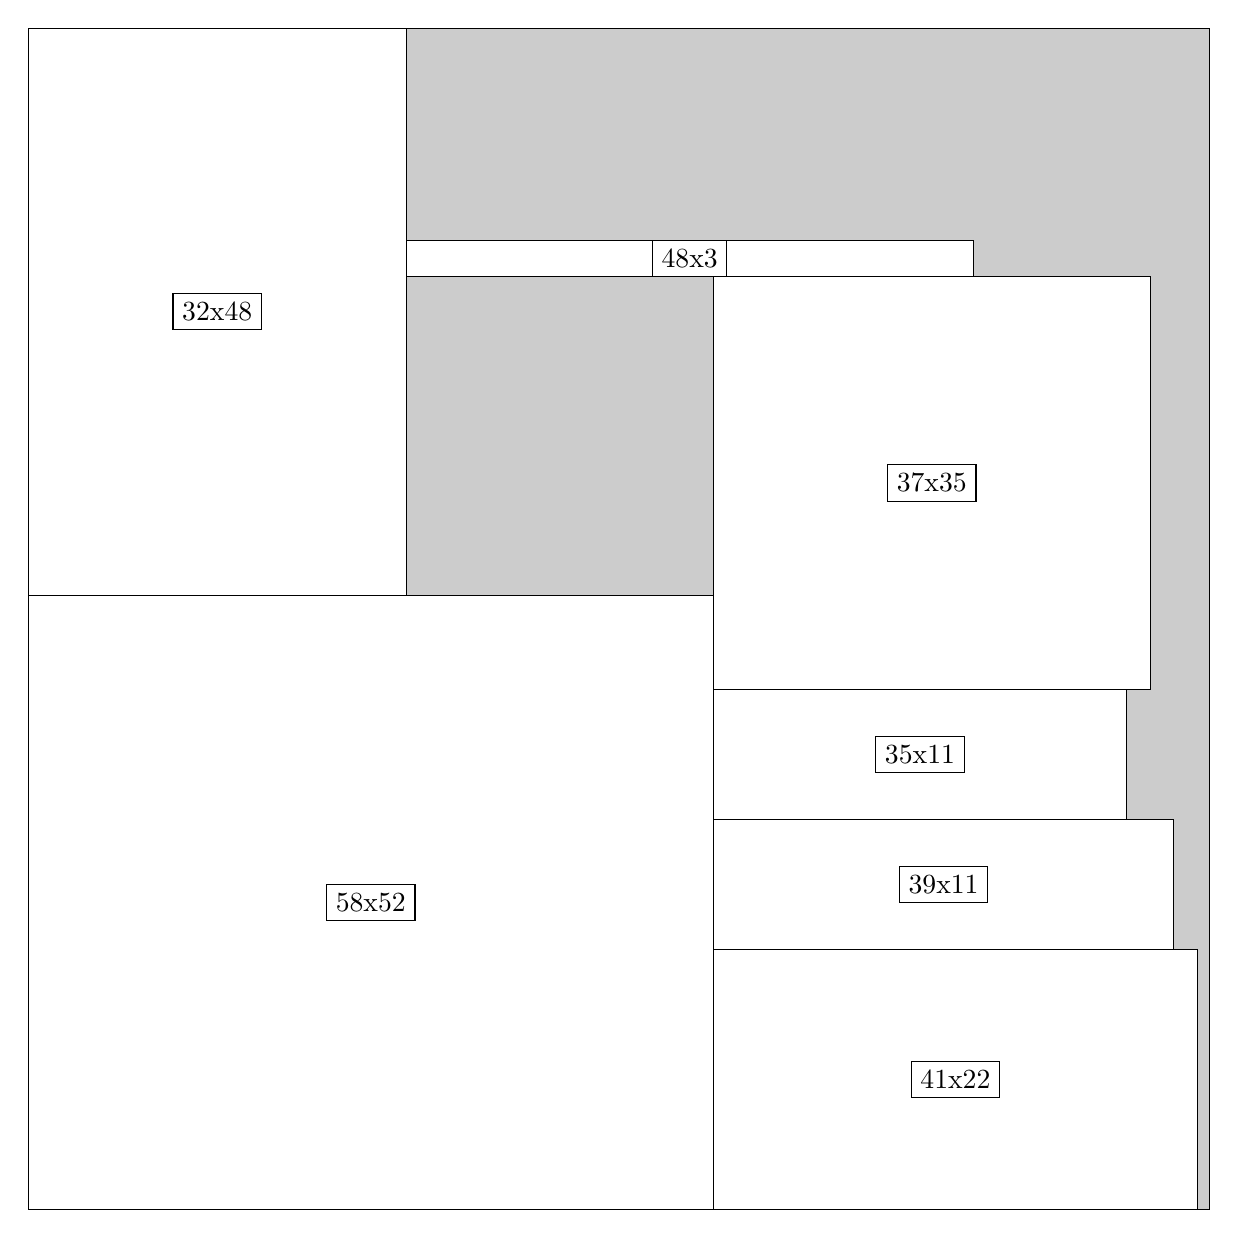
\begin{tikzpicture}[shorten >=1pt,scale=1.0,every node/.style={scale=1.0},->]
\tikzstyle{vertex}=[circle,fill=black!25,minimum size=14pt,inner sep=0pt]
\filldraw[fill=gray!40!white, draw=black] (0,0) rectangle (15.0,15.0);
\foreach \name/\x/\y/\w/\h in {58x52/0.0/0.0/8.7/7.8,32x48/0.0/7.8/4.8/7.199999999999999,37x35/8.7/6.6/5.55/5.25,41x22/8.7/0.0/6.1499999999999995/3.3,39x11/8.7/3.3/5.85/1.65,35x11/8.7/4.95/5.25/1.65,48x3/4.8/11.85/7.199999999999999/0.44999999999999996}
\filldraw[fill=white!40!white, draw=black] (\x,\y) rectangle node[draw] (\name) {\name} ++(\w,\h);
\end{tikzpicture}


w =58 , h =52 , x =0 , y =0 , v =3016
\par
w =32 , h =48 , x =0 , y =52 , v =1536
\par
w =37 , h =35 , x =58 , y =44 , v =1295
\par
w =41 , h =22 , x =58 , y =0 , v =902
\par
w =39 , h =11 , x =58 , y =22 , v =429
\par
w =35 , h =11 , x =58 , y =33 , v =385
\par
w =48 , h =3 , x =32 , y =79 , v =144
\par
\newpage


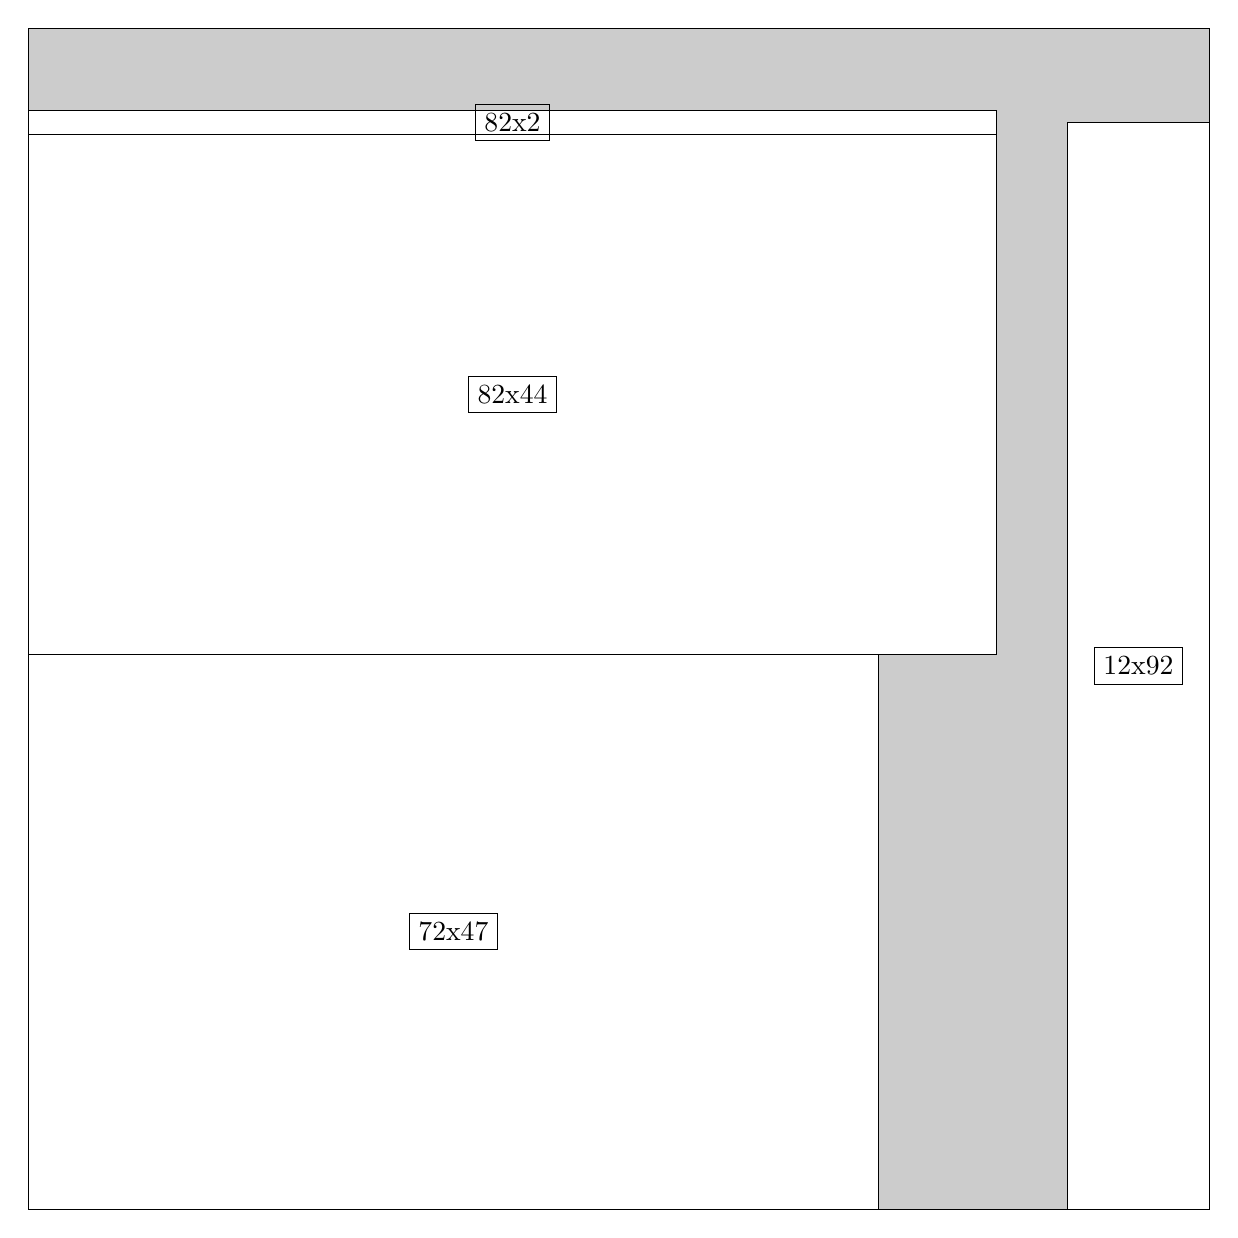
\begin{tikzpicture}[shorten >=1pt,scale=1.0,every node/.style={scale=1.0},->]
\tikzstyle{vertex}=[circle,fill=black!25,minimum size=14pt,inner sep=0pt]
\filldraw[fill=gray!40!white, draw=black] (0,0) rectangle (15.0,15.0);
\foreach \name/\x/\y/\w/\h in {72x47/0.0/0.0/10.799999999999999/7.05,82x44/0.0/7.05/12.299999999999999/6.6,12x92/13.2/0.0/1.7999999999999998/13.799999999999999,82x2/0.0/13.65/12.299999999999999/0.3}
\filldraw[fill=white!40!white, draw=black] (\x,\y) rectangle node[draw] (\name) {\name} ++(\w,\h);
\end{tikzpicture}


w =72 , h =47 , x =0 , y =0 , v =3384
\par
w =82 , h =44 , x =0 , y =47 , v =3608
\par
w =12 , h =92 , x =88 , y =0 , v =1104
\par
w =82 , h =2 , x =0 , y =91 , v =164
\par
\newpage


\end{document}